\section{Verification}\label{sec:verification}

\subsection{The test suite}
The automated suite has 663 tests in 20 modules (\tabref{tab:tests}). Except for the optional
real-GitHub tests, they run the real \code{Vault} against a simulated GitHub: an in-memory model of
the endpoints GhostVault uses that keeps what decides correctness, namely content-addressed blobs with
real Git ids, immutable trees and commits, branch updates that must fast-forward, recursive listings
and their truncation, empty repositories that answer 409 until initialised, private, archived and
read-only repositories, and tokens that stop working. A deletion is a new commit, so deleted blobs
stay in the history, as on GitHub. Nothing touches the network.

\begin{table*}[t]
\caption{The test modules}\label{tab:tests}
\centering\footnotesize
\setlength{\tabcolsep}{4pt}
\begin{tabularx}{\textwidth}{@{}L{25mm}rY@{\hspace{10pt}}L{25mm}rY@{}}
\toprule
\textbf{Module} & \textbf{Tests} & \textbf{What it checks} & \textbf{Module} & \textbf{Tests} & \textbf{What it checks} \\
\midrule
\code{resilience} & 90 & retries, backoff, rate limits, pacing, uncertain outcomes, transport, fault schedules & \code{credentials} & 30 & keychain selection, session fallback, accepted repositories \\ \addlinespace[1.6pt]
\code{gui} & 58 & the real Tk window: background work, layout, scaling, keyboard, secrets & \code{placement} & 24 & distributed and consolidated placement \\ \addlinespace[1.6pt]
\code{security} & 53 & tampered and damaged records, what decryption binds, malicious input, leaks & \code{local\_state} & 23 & the data folder, permissions, damage, the lock \\ \addlinespace[1.6pt]
\code{original\_file} & 51 & which files are accepted; reading safely; the deletion race & \code{gallery} & 17 & encrypted previews and renaming \\ \addlinespace[1.6pt]
\code{recovery} & 49 & recovery files and the repository backup, end to end & \code{restore\_safety} & 16 & never replacing a file; flushing before remote deletion \\ \addlinespace[1.6pt]
\code{packaging} & 43 & the build script, the PyInstaller specification, the install scripts & \code{compatibility} & 16 & records of format 5, written by an earlier version's own code \\ \addlinespace[1.6pt]
\code{journal} & 41 & an interruption at each checkpoint, then start-up recovery & \code{real\_github} & 14 & optional: the same operations on real repositories \\ \addlinespace[1.6pt]
\code{units} & 41 & helpers, atomic writes, start-up, self-check, TLS & \code{remote\_cleanup} & 13 & removal that GitHub refuses or applies only in part \\ \addlinespace[1.6pt]
\code{ghost\_and\_restore} & 38 & the core cycle and its failure modes & \code{github\_layer} & 10 & what the GitHub layer verifies; streaming without staging \\ \addlinespace[1.6pt]
\code{backup\_integrity} & 31 & incomplete records never shrink a backup & \code{logging} & 5 & the log never holds an exception's message \\
\bottomrule
\end{tabularx}
\end{table*}

Four techniques carry most of the weight.
\emph{Simulated crashes:} a test harness stops the vault at a named checkpoint by raising an exception
that none of GhostVault's error handling catches, as when a process dies; it then starts a new vault on
the same folder, runs start-up recovery, and checks that the file is in at least one place byte for
byte (the original, a restorable ghost, or the restored file), that every chunk on GitHub is accounted
for by a record, and that no temporary file is left. Every checkpoint in the code is covered.
\emph{Faults:} requests fail before GitHub acts or after it acted with the reply lost, on schedules that
are a pure function of a seed and the request itself, so parallel downloads cannot change which
requests fail and every run is exactly reproducible.
\emph{Property tests:} seeded random damage to recovery files (300 cases) and records (250 cases)
must be refused or fail closed, never give wrong bytes; padding is checked at 40 random sizes.
\emph{The real interface:} the GUI tests drive the Tk window itself (under Xvfb on Linux) and are
written to hold on Tk 8.6 and Tk 9 and at any display scale.

The suite checks outcomes, not the absence of exceptions: the bytes restored, the original still
present, what is on the simulated GitHub, file modes, and what the user is told. The real-GitHub tests
run only with dedicated repositories and a token supplied in the environment.

\subsection{Crashes and faults together}\label{sec:stress}
A separate tool, \code{tools/stress.py}, runs long random sequences of operations against the
simulated GitHub with two repositories and a 4\,KiB chunk size, so that files have many chunks. Each
cycle ghosts a new random file (of a size chosen among the edge cases 0, 1, 4\,095, 4\,096 and
4\,097 bytes and random sizes up to twelve chunks, with random placement and padding) or restores a
random ghost. With a given probability the operation is stopped at a random checkpoint and GhostVault
is restarted on the same folder; network faults are injected throughout, transient as on a real
network (no request fails more than three times in a row). After every cycle the invariants of the
crash tests are checked; at the end every ghost is restored, start-up recovery runs once more, and
GitHub must hold no chunk at all.

Eight runs were made: five with a crash probability of 0.35 and a fault rate of 0.05, and three with
0.5 and 0.15, 400 cycles each. Together they executed 3\,200 operations, stopped 1\,273 of them at a
checkpoint (\figref{fig:crashes}), injected 7\,736 network faults, ran start-up recovery 1\,273 times
and checked the invariants 3\,208 times. Every invariant held in every run: no file was lost, no chunk
was left unaccounted for, every ghost restored byte for byte, and GitHub was empty at the end. The runs
took 61\,s in total. This test stops the process at checkpoints; the file system itself stays
consistent, so it does not simulate a power failure, which the ordering of flushes
(\secref{sec:durable}) is designed for but which was not tested.

\begin{figure}[t]
\centering
% Fig.: simulated crashes per checkpoint in the stress runs (report/data/stress.json), in the
% order the checkpoints are reached.
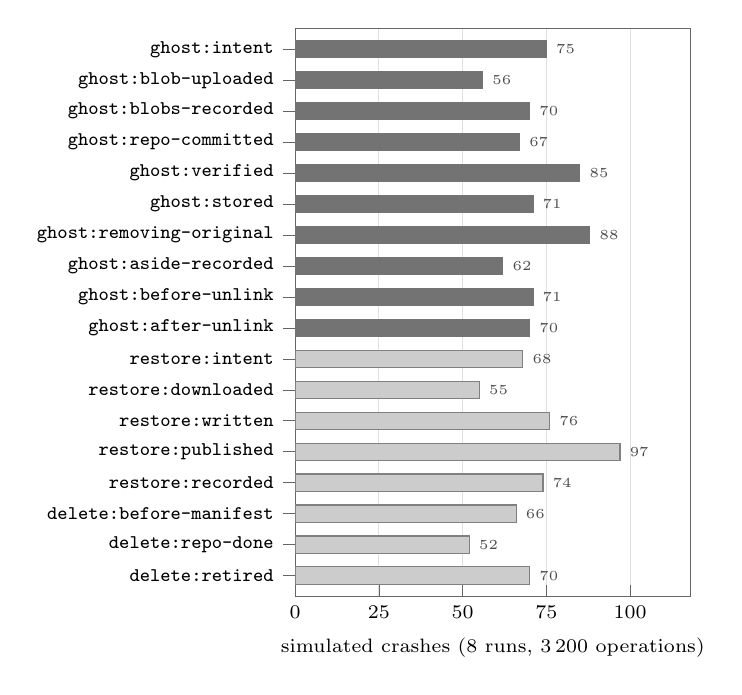
\begin{tikzpicture}
\begin{axis}[
  xbar, bar shift=0pt, width=66mm, height=88mm,
  font=\scriptsize,
  bar width=2.2mm,
  xmin=0, xmax=118, xtick={0,25,50,75,100},
  xlabel={simulated crashes (8 runs, 3\,200 operations)},
  y dir=reverse, enlarge y limits=0.04,
  ytick={ghost:intent, ghost:blob-uploaded, ghost:blobs-recorded, ghost:repo-committed,
                     ghost:verified, ghost:stored, ghost:removing-original, ghost:aside-recorded,
                     ghost:before-unlink, ghost:after-unlink, restore:intent, restore:downloaded,
                     restore:written, restore:published, restore:recorded, delete:before-manifest,
                     delete:repo-done, delete:retired},
  xtick pos=bottom, ytick pos=left,
  symbolic y coords={ghost:intent, ghost:blob-uploaded, ghost:blobs-recorded, ghost:repo-committed,
                     ghost:verified, ghost:stored, ghost:removing-original, ghost:aside-recorded,
                     ghost:before-unlink, ghost:after-unlink, restore:intent, restore:downloaded,
                     restore:written, restore:published, restore:recorded, delete:before-manifest,
                     delete:repo-done, delete:retired},
  yticklabel style={font=\scriptsize\ttfamily},
  axis line style={black!60}, tick style={black!60},
  xmajorgrids, grid style={black!12},
  nodes near coords, nodes near coords style={font=\tiny, text=black!70, anchor=west},
]
\addplot[fill=black!55, draw=black!55] coordinates {
  (75,ghost:intent) (56,ghost:blob-uploaded) (70,ghost:blobs-recorded) (67,ghost:repo-committed)
  (85,ghost:verified) (71,ghost:stored) (88,ghost:removing-original) (62,ghost:aside-recorded)
  (71,ghost:before-unlink) (70,ghost:after-unlink)};
\addplot[fill=black!20, draw=black!50] coordinates {
  (68,restore:intent) (55,restore:downloaded) (76,restore:written) (97,restore:published)
  (74,restore:recorded) (66,delete:before-manifest) (52,delete:repo-done) (70,delete:retired)};
\end{axis}
\end{tikzpicture}

\caption{Where the stress runs stopped the process: the 18 checkpoints of ghosting (dark) and of
restoring and removing (light), in the order they are reached. Data: \code{report/data/stress.json}.}
\label{fig:crashes}
\end{figure}

\subsection{What was verified, and where}\label{sec:status}
\tabref{tab:status} lists what was run for the version this report describes, on what, and with what
result. All of it ran on one Linux x86-64 machine. Windows and macOS were not available there,
GitHub Actions was not run, PyInstaller could not be installed for lack of access to the package
index, and no real GitHub repository was used.

\begin{table*}[t]
\caption{Verification status of GhostVault 1.0.0}\label{tab:status}
\centering\footnotesize
\begin{tabularx}{\textwidth}{@{}L{60mm}L{50mm}Y@{}}
\toprule
\textbf{What} & \textbf{Where} & \textbf{Result} \\
\midrule
The test suite, Python 3.13.14 with Tk 9.0.3, under Xvfb & Linux x86-64 (Ubuntu 24.04), as root &
640 passed, 23 skipped: 14 need real GitHub, 6 Windows, 2 a non-root user, 1 the machine's keychain \\ \addlinespace[1.6pt]
The test suite, Python 3.11 and 3.14 with Tk 9.0 & the same & 638 passed, 2 failed, 23 skipped each; both failures from this machine's builds of the dependencies (below) \\ \addlinespace[1.6pt]
The test suite, Python 3.12 with Tk 8.6.15 & the same & the same as for 3.11 and 3.14 \\ \addlinespace[1.6pt]
The test suite as an unprivileged user, Python 3.13 & the same & not completed (run stopped) \\ \addlinespace[1.6pt]
The core without Tk (system Python 3.13, no \code{tkinter}) & the same & 575 passed, 86 skipped (GUI), 2 failed as above \\ \addlinespace[1.6pt]
Lint: \code{ruff}; \code{shellcheck} on the install scripts; \code{actionlint} (with
\code{shellcheck}) on the three workflows & the same & no findings \\ \addlinespace[1.6pt]
The wheel: built, contents checked, installed into an empty environment and started & the same &
not run for this version \\ \addlinespace[1.6pt]
The PyInstaller specification: executed with stand-ins for PyInstaller under Linux, Windows and
macOS settings; type-checked against PyInstaller's type stubs & the same & spec tests passed; type check not run for this version \\ \addlinespace[1.6pt]
\code{build.py} after freezing (smoke test, packaging, verification with install, update and
uninstall), on a stand-in for PyInstaller's output folder & the same & not run for this version \\ \addlinespace[1.6pt]
The stress runs (\secref{sec:stress}) and the measurements (\secref{sec:performance}) & the same,
Python 3.13 & every invariant held; measurements as reported \\
\midrule
\multicolumn{3}{@{}p{\textwidth}@{}}{\emph{The two failures outside Python 3.13 are environmental: the Pillow built here for
those interpreters has no JPEG encoder, which \code{--self-check} rightly reports as missing; and the
\code{packaging} distribution was absent, so a test imported the project's own \code{packaging/} folder
instead (the test now skips in that case).}} \\ \addlinespace[1.6pt]
\midrule
The test suite on Windows and macOS (the CI matrix) & --- & not run \\ \addlinespace[1.6pt]
The real-GitHub tests & --- & not run \\ \addlinespace[1.6pt]
PyInstaller itself, the standalone applications, the Windows installer, the disk images, code
signing, notarization, and the release workflow & --- & not run \\
\bottomrule
\end{tabularx}
\end{table*}
